\documentclass[12pt]{article}
\usepackage{amsmath}
\usepackage{amsthm}
\usepackage{amssymb}
\usepackage{amsfonts}
\usepackage[width=12cm,left=2cm,top=3cm]{geometry}
\usepackage{graphicx}
\usepackage{bookmark}
\usepackage{tikz-cd}
\usepackage{hyperref}

\usepackage{tikz}
\usetikzlibrary{automata,positioning}

\theoremstyle{definition}
\newtheorem{definition}{Definition}[section]
\newtheorem{thm}[definition]{Theorem}
\newtheorem{proposition}[definition]{Proposition}
\newtheorem{corollary}[definition]{Lemma}
\newtheorem{lemma}[definition]{Corollary}

% \theoremstyle{plain} 
\newtheorem{exam}[definition]{Example}
\theoremstyle{remark}
\newtheorem{remark}[definition]{Remark}

\newcommand{\ip}[2]{(#1,#2)}
\font\ninerm=cmr9

\begin{document}
\title{Pushdown automata}   
\maketitle 
A pushdown automata is a type of automation that use a stack structure, with the remaining part the same as the NFA (non-definite finte state automata). With the repect to the stack the pushdown automata has gained a more greater ability to describe the language. We will in the further section prove that pushdown automata has just the same ability describing as Context free grammar. 

\section{The definition of PDA}
\label{sec:The definition of PDA}

What is new in the pushdown automata is that there is a stack that we can operate when we receive a character. 
When it receive a character of \( \Sigma\), the automata is going to next state based on three object: 1. the current state; 2. the received character of \( \Sigma\); 2. the character on the top of the stack. 

If you wrote out the defintion of state-transition function, it would be something like: \(\delta \colon Q \times \Sigma \times Z \to Q\), where \(Z\) denote the character in the stack (and of course that \(Z\) can equate \(Q\)). 

Let's take the pushdown automata that describe the language \(L = \{ w w ^{R} \}\) as an example. 

\begin{exam}
	{\sl
It is clear that we should push \(a\) into the stack if we receive \(a\), before we finish going through the string \(w\). And it is the same clear that we should get the top of the stack and check if it is the same as the received character after we go through the string \(w\).

The tricky one is that we have to check these two kinds of situation at the same time, for that every time we get a character, it could be that the \(w\) is done or not.

We can use NFA with two state to construct the pushdown automaton we need.

We say that the automata is at \(q_{0}\) saying that we are at \(w\), and the state \(q_1\) is saying that we are at \(w ^{R}\). And before we receive a character we use a \(\epsilon\) transition from \(q_{0}\) to \(q_1\),
after figuring out which, all is clear.
}
\begin{figure}
	\centering
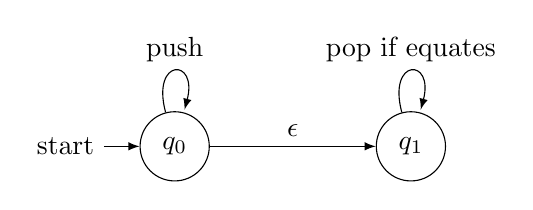
\begin{tikzpicture}[>=latex,node distance=3cm,on grid,auto]
   \node[state,initial] (q_0)   {$q_0$};
   \node[state] (q_1) [right=of q_0] {$q_1$};
    \path[->]
    (q_0) edge  node {\(\epsilon\)} (q_1)
          edge [loop above] node {push} ()
	(q_1) edge [loop above] node {pop if equates} ();
\end{tikzpicture}
\end{figure}
\end{exam}

\subsection{The precise definition of the pushdown automata}
A pushdown automaton is a seven tuple: \(P = (Q , \Sigma , \Gamma ,\delta , q_{0}, Z _{0} , F)\). 
\begin{quotation}
	\( \Gamma\) is the set of the character that appears in the stack 

	\smallskip
	\( Z _{0}\) is the initial character that located in the stack. 

	\smallskip
	Moreover, the state-transition function should be like: 
	\[
		\delta _{0} \colon Q \times \Sigma \times \Gamma \to \mathfrak P (Q)
	\]
	for that the the pushdown automata is built on a NFA.
\end{quotation}
Also, the element on the top of the stack is always popped. If you want the stack to remain un-changed, you can define something like \(\delta (q_{i}, a,\alpha) = \{ \ip {q_{j}}\alpha \}\) 


\begin{exam}
Let us just skip the blahblah and draw a diagram that shows how a pushdown automaton work. 
\begin{figure}
	\centering
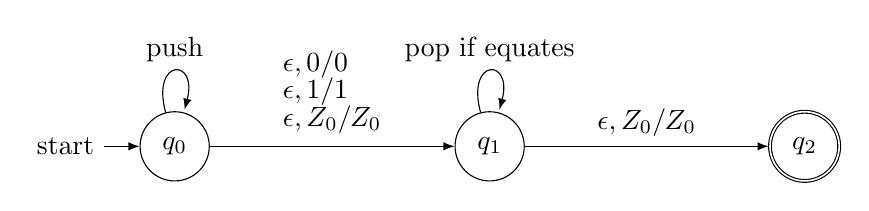
\begin{tikzpicture}[>=latex,node distance=4cm,on grid,auto]
   \node[state,initial] (q_0)   {$q_0$};
   \node[state] (q_1) [right=of q_0] {$q_1$};
   \node[state,accepting] (q_2) [right=of q_1] {\(q_{2}\)}; 
    \path[->]
	(q_0) edge  node { \(%
	\begin{aligned}% 
		&\epsilon, 0 / 0 \\[-5pt]
		&\epsilon , 1 / 1 \\[-5pt]
		&\epsilon , Z_{0} / Z _{0}  
	\end{aligned}\) } (q_1)
          edge [loop above] node {push} ()
	(q_1) edge [loop above] node {pop if equates} ()
	      edge node { \(\epsilon, Z _{0} / Z_{0}\)} (q_2);
\end{tikzpicture}
\end{figure}
\end{exam}
% subsection:The precise definition of the pushdown automata 

\subsection{Instantaneous Descriptions of a Pushdown automata}
We introduce the instantaneous descriptions of PDA to show how 
a PDA accept a string. 

A string is given and the string is the 
input of the PDA. What will happen in the PDA is that part of 
the string is received and state changes and stack is pushed into 
character or the other way. Then the information in the middle of 
the procedure contains three parts: 1. the state; 2. the string in 
the stack; 3. the remaining string. 
\begin{enumerate}
\item the state
\item the string in stack
\item the remaining string
\end{enumerate}
So we can describe the middle state of the whole PDA with a three 
tuple---\((q, w ,\gamma)\), where \(q \in Q\), \( w\in \Sigma ^{*} \), \(\gamma \in \Gamma ^{*}\). We use \(\vdash\) to indicate that 
an ID can transit to the other. Then we know that if \(\delta (q , a , X )\) contains \( ( p ,\alpha)\) we will know that 
\[
	(q , a w , X\beta ) \vdash ( p , w ,\alpha \beta )
\]
It is very similar to the function \( \hat\delta\) in the finite state automata. And it is very similar to the symbol \( \Rightarrow\)
in the context free grammar.   Similarly we use \( \overset{*}{\vdash}\) to indicate that one ID can transit to the other after zero or one or more
than one character are received. 

If \((q_{1} , w_{1} ,\gamma _{1}) \vdash ^{*} (q_{2}, w_2,\gamma_2)\) then
\((q_{1} , w_{1} ,\gamma _{1}) \sim (q_{2}, w_2,\gamma_2)\)


\begin{thm}[Deduction principle]
\label{Deduction principle}
	\(P  = ( Q , \Sigma , \Gamma ,\delta , q _{0}, Z _{0}, F)\)
	is a PDA. If \((q , x ,\alpha )\vdash ^{*} ( p, y  ,\beta)\) , then 
	\[
		(q,  x w ,\alpha \gamma ) \vdash ^{*} (p , y w, \beta \gamma)
	\]
\end{thm}
% theorem Deduction principle 

\begin{proof}
The proof is trivial. 
\end{proof}
However, it is worth noting that the converse of the thm is not 
true. 
% subsection:Instantaneous Descriptions of a Pushdown automata 

% section The definition of PDA 
\end{document}      
